\documentclass[11pt]{article}
\usepackage{color, array, graphics}
\usepackage{amsmath}
\usepackage{amssymb}
\usepackage{enumerate}
\usepackage{mathtools}
\usepackage{fullpage}
\usepackage{graphicx}
\usepackage[utf8]{inputenc}
\usepackage{tikz}

%Symbol shortcuts
\def\OR{\vee}
\def\AND{\wedge}
\def\imp{\rightarrow}

%Aesthetics
\addtolength{\oddsidemargin}{-.5in}
\addtolength{\evensidemargin}{-.5in}

\addtolength{\topmargin}{-.5in}

\begin{document}

\textbf{Alexander Garcia}

5 May 2017 \\

	\begin{enumerate}

			\item Question 1

				\begin{enumerate}[(a)]

					\item

						$S \rightarrow 00S1$

						$S \rightarrow 1S00$

						The first two are clear rules of the language. When adding a single 1,
						you must also add two 0's \\

						$S \rightarrow SS$

						Concatenating two existing strings in the grammar will also produce a vaild string.
						Both have the correct relationship between 1's and 0's, so the relationship does not
						change when they are combined \\


						$S \rightarrow 0S1S0$

						The forth rule allows the concatenation of two existing strings, and adding two 0's and a 1,
						allowing for ``random'' placement of 1's and 0's. \\


						$S \rightarrow \lambda$

						The fifth rule allows for the termination of a derivation \\

					\item 	\begin{tabular}{ll}

						$S \rightarrow 00S1$ & Rule 1 \\

						$00S1 \rightarrow 00[1S00]1$ & Rule 2 \\

						$00[1S00]1 \rightarrow 00[1[0S1S0]00]1$ & Rule 4 \\

						$00[1[0S1S0]00]1 \rightarrow 001010001$ & Rule 5 for both $S$ \\

					\end{tabular}

				\end{enumerate}

				\newpage

				\textbf{Alexander Garcia}

				5 May 2017 \\

			\item Question 2

			\begin{center}
				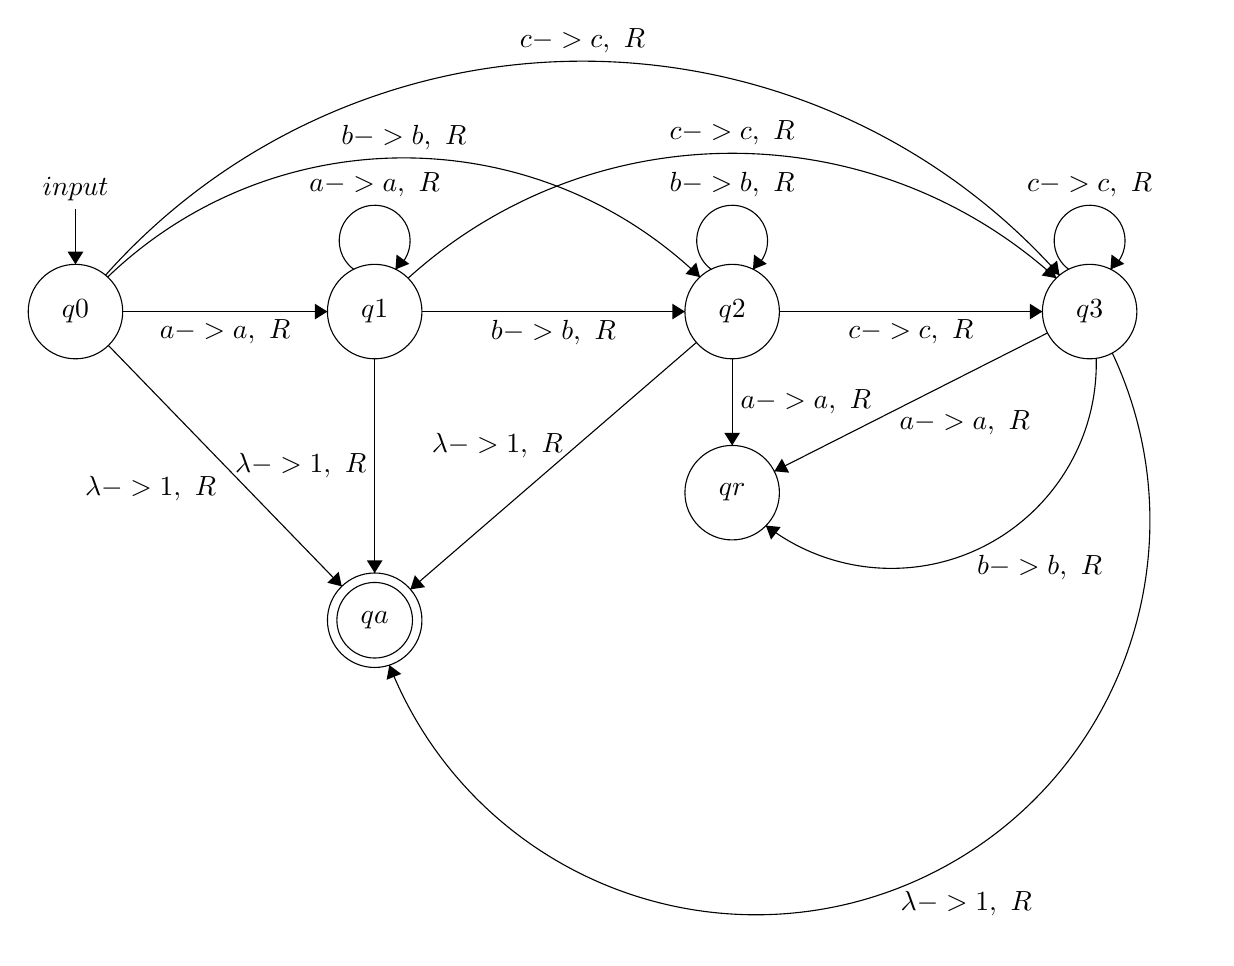
\begin{tikzpicture}[scale=0.2]
					\tikzstyle{every node}+=[inner sep=0pt]
					\draw [black] (5.1,-18.8) circle (3);
					\draw (5.1,-18.8) node {$q0$};
					\draw [black] (24.1,-18.8) circle (3);
					\draw (24.1,-18.8) node {$q1$};
					\draw [black] (46.8,-18.8) circle (3);
					\draw (46.8,-18.8) node {$q2$};
					\draw [black] (69.5,-18.8) circle (3);
					\draw (69.5,-18.8) node {$q3$};
					\draw [black] (46.8,-30.3) circle (3);
					\draw (46.8,-30.3) node {$qr$};
					\draw [black] (24.1,-38.4) circle (3);
					\draw (24.1,-38.4) node {$qa$};
					\draw [black] (24.1,-38.4) circle (2.4);
					\draw [black] (5.1,-12.3) -- (5.1,-15.8);
					\draw (5.1,-11.8) node [above] {$input$};
					\fill [black] (5.1,-15.8) -- (5.6,-15) -- (4.6,-15);
					\draw [black] (8.1,-18.8) -- (21.1,-18.8);
					\fill [black] (21.1,-18.8) -- (20.3,-18.3) -- (20.3,-19.3);
					\draw (14.6,-19.3) node [below] {$a->a,\mbox{ }R$};
					\draw [black] (7.145,-16.607) arc (133.84128:46.15872:27.149);
					\fill [black] (44.76,-16.61) -- (44.52,-15.69) -- (43.83,-16.41);
					\draw (25.95,-8.54) node [above] {$b->b,\mbox{ }R$};
					\draw [black] (7.01,-16.488) arc (138.32307:41.67693:40.554);
					\fill [black] (67.59,-16.49) -- (67.43,-15.56) -- (66.68,-16.22);
					\draw (37.3,-2.4) node [above] {$c->c,\mbox{ }R$};
					\draw [black] (27.1,-18.8) -- (43.8,-18.8);
					\fill [black] (43.8,-18.8) -- (43,-18.3) -- (43,-19.3);
					\draw (35.45,-19.3) node [below] {$b->b,\mbox{ }R$};
					\draw [black] (49.8,-18.8) -- (66.5,-18.8);
					\fill [black] (66.5,-18.8) -- (65.7,-18.3) -- (65.7,-19.3);
					\draw (58.15,-19.3) node [below] {$c->c,\mbox{ }R$};
					\draw [black] (26.221,-16.681) arc (132.16921:47.83079:30.654);
					\fill [black] (67.38,-16.68) -- (67.12,-15.77) -- (66.45,-16.51);
					\draw (46.8,-8.25) node [above] {$c->c,\mbox{ }R$};
					\draw [black] (46.8,-21.8) -- (46.8,-27.3);
					\fill [black] (46.8,-27.3) -- (47.3,-26.5) -- (46.3,-26.5);
					\draw (47.3,-24.55) node [right] {$a->a,\mbox{ }R$};
					\draw [black] (69.918,-21.764) arc (1.43071:-127.69644:13.019);
					\fill [black] (48.94,-32.39) -- (49.27,-33.28) -- (49.88,-32.48);
					\draw (66.32,-34.22) node [below] {$b->b,\mbox{ }R$};
					\draw [black] (66.82,-20.16) -- (49.48,-28.94);
					\fill [black] (49.48,-28.94) -- (50.42,-29.03) -- (49.96,-28.14);
					\draw (61.57,-25.06) node [below] {$a->a,\mbox{ }R$};
					\draw [black] (24.1,-21.8) -- (24.1,-35.4);
					\fill [black] (24.1,-35.4) -- (24.6,-34.6) -- (23.6,-34.6);
					\draw (23.6,-28.6) node [left] {$\lambda->1,\mbox{ }R$};
					\draw [black] (7.19,-20.95) -- (22.01,-36.25);
					\fill [black] (22.01,-36.25) -- (21.81,-35.32) -- (21.1,-36.02);
					\draw (14.07,-30.07) node [left] {$\lambda->1,\mbox{ }R$};
					\draw [black] (44.53,-20.76) -- (26.37,-36.44);
					\fill [black] (26.37,-36.44) -- (27.3,-36.3) -- (26.65,-35.54);
					\draw (31.89,-28.11) node [above] {$\lambda->1,\mbox{ }R$};
					\draw [black] (70.938,-21.431) arc (25.21883:-158.51737:25.016);
					\fill [black] (25.03,-41.25) -- (24.86,-42.18) -- (25.79,-41.81);
					\draw (61.67,-55.6) node [below] {$\lambda->1,\mbox{ }R$};
					\draw [black] (22.777,-16.12) arc (234:-54:2.25);
					\draw (24.1,-11.55) node [above] {$a->a,\mbox{ }R$};
					\fill [black] (25.42,-16.12) -- (26.3,-15.77) -- (25.49,-15.18);
					\draw [black] (45.477,-16.12) arc (234:-54:2.25);
					\draw (46.8,-11.55) node [above] {$b->b,\mbox{ }R$};
					\fill [black] (48.12,-16.12) -- (49,-15.77) -- (48.19,-15.18);
					\draw [black] (68.177,-16.12) arc (234:-54:2.25);
					\draw (69.5,-11.55) node [above] {$c->c,\mbox{ }R$};
					\fill [black] (70.82,-16.12) -- (71.7,-15.77) -- (70.89,-15.18);
				\end{tikzpicture}
			\end{center}

			The diagram of this machine is quite complicated so this is a summary of its functionality.

			The string starts accepting input. Any character in the alphabet, including $\lambda$, is sent to a
			specific state. If a letter that comes after the first letter is seen, the machine immediately goes to the reject state.
			If the same letter is seen, it stays in the previous state. If a ``higher'' letter is seen, it goes to that letter's state.

			As long as the sequence is lexographic, the machine will stay in one of the three letters' states during the whole input, not
			modifying the input in any way. When a blank space is seen, if the machine is in one of the three states, it will write a 1, and
			enter the accept state. \\

			\newpage

			\textbf{Alexander Garcia}

			5 May 2017 \\

		\item Question 3

			\begin{enumerate}[(a)]

				\item The main idea behind this machine is to erase pairs of 1's and 0's. \\

					Start cycling through the tape. If you see a 1, remove it, then continue cycling until you reach a
					0 or the end. If you reach a 0, remove it as well, and start searching for another 1, repeating the process. \\

					If you reach the end of the input string, start over at the beginning and repeat the process of removing one 1, skipping
					to the next 0, then removing that 0. If you are able to make it to the end of the tape without removing any digits, you have
					reached a conclusion. If there are only 0's left, the machine enters the accept state, as there were more 0's than 1's. If there
					are no digits left, there were exactly as many 0's as there were 1's, and the machine enters the reject state, as it only recognizes
					words with more 0's than 1's. If there are 1's remaining, it enters the reject state also. \\

				\item The runtime of this machine is as follows.

					$r = n + m$

					m = number of 1's, n = number of 0's, r = length of the string

					The worst case runtime would be if there are equal numbers of 1's and 0's, or $m=n=\frac{r}{2}$. Because of the way this machine
					operates, the worst case order of digits would be $\frac{r}{2} 1$'s followed by $\frac{r}{2} 0$'s, as the machine would then only
					remove 2 items per pass.

					So, the machine would read $r$ digits the first pass, $r-2$ digits the second pass, $r-4$ the third, and so on.

					This summation is $\sum_{i=1}^{r/2}{r-2j} = \frac{1}{4} (r-2)*r$

					In terms of order notation, this makes the algorithm $O(r^2)$ \\

			\end{enumerate}

			\newpage

			\textbf{Alexander Garcia}

			5 May 2017 \\

		\item Question 4

		\begin{enumerate}[(a)]

			\item $L = \{w\#w^R\#w |w \in \{a,b\}^+\}$

				Assuming the input string $w$ is on a single tape, and there is one empty string for reading/writing

				\begin{enumerate}[(1)]

					\item 	Jump across the tape, going from the first position on the input tape to the first
						position after the 2nd $\#$

					\item 	Repeat this process until the left side reaches a break ($\#$)

					\item 	If the two sides differ at any point, reject the input, as the string does not appear on
						either side of two $\#$s

					\item 	If each side had the same symbol up to that point, start working backwards from the
						$\#$ to the start of the input tape, writing the character to the head of the second tape

					\item 	Iterate through the input tape again, starting this time from the first position after the
						first $\#$. Compare these inputs to those written to the secondary tape until the next
						$\#$ is reached. If they differ at any point, reject the input. If they are identical,
						accept the input \\

				\end{enumerate}

			\item Worst case runtime for this machine

				The machine searches for a pattern of length $w$. For each string it tests (input up to the first $\#$), it
				must test another string of the same length, checking the string will in fact repeat. It must then read
				backwards through $w$ positions while it writes to the second tape. It then compares $w$ characters from the
				reversed string to the middle segment.

				One cycle = (beginning string + repeated string) + backwards read/write + middle compare

				$O(w) = 4w$

		\end{enumerate}
			\newpage

			\textbf{Alexander Garcia}

			5 May 2017 \\

		\item Question 5

			In order for $\mathbb{N} \times \mathbb{N}$ to be countable, every pair of numbers $(\mathbb{N}, \mathbb{N})$ must
			map to a unique element of $\mathbb{N}$

			$\mathbb{N}$ is countable by definition, since a set is countable if every element in the set can be mapped to
			$\mathbb{N}$

			Take a number $k = 2^x*3^y$ where $k,x,y \in \mathbb{N}$

			According to the fundamental theorem of arithmetic, this is the only prime factorization of $k$, and therefore
			the only possible values of $x$ and $y$

			We treat this as the function $f(x,y) = 2^x*3^y$

			$x,y$ are each in the domain $\mathbb{N}$, giving the function $f(x,y)$ the domain of $\mathbb{N}^2$

			The right side of the function maps each combination of $(x,y)$ to a single value of $\mathbb{N}$

			The function maps $\mathbb{N}^2 \rightarrow \mathbb{N}$

			\begin{center}
			$\therefore \mathbb{N} \times \mathbb{N}$ is countable
			\end{center}

	\end{enumerate}

\end{document}


